\documentclass[aspectratio=169]{beamer}

\PassOptionsToPackage{table}{xcolor}

\usepackage[T2A]{fontenc}
\usepackage[utf8]{inputenc}
\usepackage[main=russian,english]{babel}
\usepackage{graphicx}
\usepackage{booktabs}
\usepackage{tabularx}
\usepackage{amsmath}
\usepackage{tikz}
\usepackage{colortbl}

\usetikzlibrary{shapes.geometric,positioning}

\usetheme{Madrid}
\usecolortheme{default}
\setbeamertemplate{navigation symbols}{}
\setbeamerfont{frametitle}{size=\Large}

\graphicspath{{images/}}

\title{Обучение с подкреплением\\для игры <<Змейка>>}
\author{Полегина А.\,Д.\\Научный руководитель: к.\,ф.-м.\,н., доцент С.\,Г.\,Красовский}
\institute{БГУ, мехмат, каф. дифф.\ уравнений и системного анализа}
\date{Минск, 2026}

\begin{document}

\begin{frame}[plain]
\titlepage
\end{frame}

\begin{frame}{Цель и задачи}
\textbf{Цель:} разработать игру <<Змейка>> на Python, реализовать Q-learning для управления агентом и оценить качество обучения.

\vspace{0.5cm}
\textbf{Задачи:}
\begin{itemize}
    \item Изучить алгоритм Q-learning
    \item Реализовать логику игры и RL-среду
    \item Задать состояние, действия и награду
    \item Провести эксперименты и проанализировать результат
\end{itemize}

\vspace{0.4cm}
\textbf{Почему <<Змейка>> + RL:} дискретная среда, мало действий, наглядный результат
\end{frame}

\begin{frame}{Сравнение подходов}
\centering
\begin{tabularx}{0.92\textwidth}{>{\raggedright\arraybackslash}p{0.22\textwidth} >{\raggedright\arraybackslash}p{0.26\textwidth} X}
    \toprule
    Подход & Плюсы & Минусы \\
    \midrule
    Правила и эвристики & Простота реализации & Слабая адаптивность \\
    Поиск траектории & Явный маршрут & Нет обучения на опыте \\
    \rowcolor{blue!15} Табличный Q-learning & Интерпретируемость, связь с дискретной средой & Масштабируемость \\
    DQN & Сложные состояния & Много ресурсов и настройки \\
    \bottomrule
\end{tabularx}

\vspace{0.5cm}
\textbf{Выбран табличный Q-learning} --- баланс простоты и пользы для учебного проекта
\end{frame}

\begin{frame}{Состояние агента: 11 бинарных признаков}
\centering
\begin{tikzpicture}[
    box/.style={draw, rounded corners, minimum width=4.5cm, minimum height=0.8cm, font=\large},
]
\node[box, fill=red!20] at (0,2.4) {danger\_straight / left / right};
\node[box, fill=blue!20] at (0,1.2) {dir\_up / down / left / right};
\node[box, fill=green!20] at (0,0) {food\_left / right / up / down};
\end{tikzpicture}

\vspace{0.3cm}
\begin{itemize}
    \item \textcolor{red!70}{3} --- опасность рядом
    \item \textcolor{blue!70}{4} --- текущее направление
    \item \textcolor{green!70}{4} --- положение пищи
\end{itemize}

\vspace{0.2cm}
Компактное описание $\Rightarrow$ подходит для табличного Q-learning
\end{frame}

\begin{frame}{Действия и награда}
\textbf{3 относительных действия:}
\begin{center}
\Large идти прямо \quad\quad повернуть влево \quad\quad повернуть вправо
\end{center}

\vspace{0.2cm}
\small Относительные --- уменьшают избыточность: <<повернуть влево>> имеет один смысл при любом направлении.

\vspace{0.4cm}
\textbf{Функция награды:}
\begin{center}
\begin{tabular}{cc}
    \toprule
    Событие & Награда \\
    \midrule
    Пища & $+10.0$ \\
    Столкновение & $-10.0$ \\
    Шаг & $-0.1$ \\
    \bottomrule
\end{tabular}
\end{center}

\vspace{0.2cm}
Штраф за шаг $\Rightarrow$ агент не движется бесконечно по кругу
\end{frame}

\begin{frame}{Архитектура программной системы}
\centering
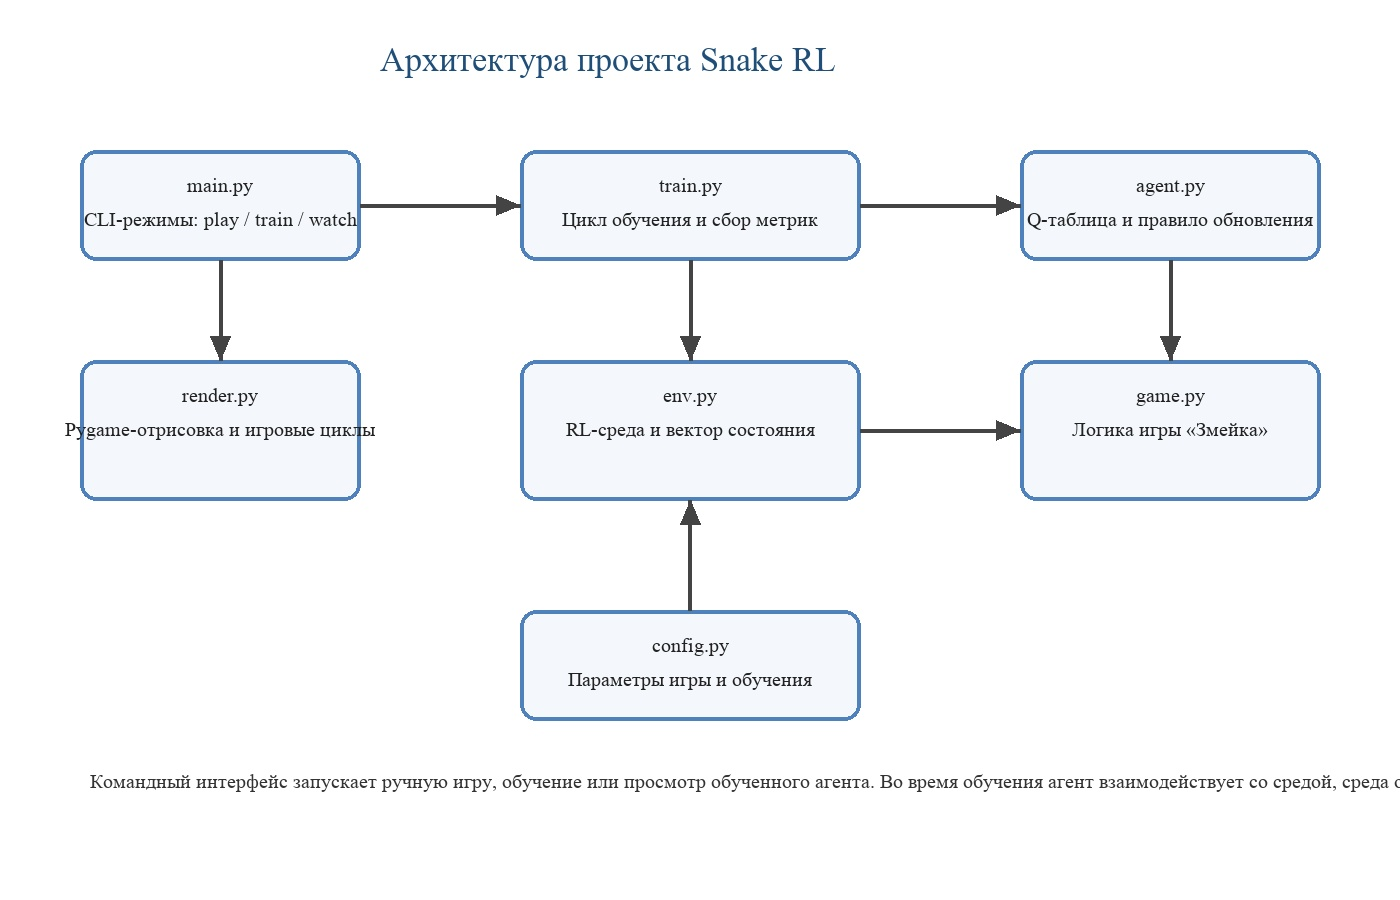
\includegraphics[width=0.85\textwidth]{images/architecture.jpg}
\end{frame}

\begin{frame}{Алгоритм Q-learning}
\begin{center}
\Large
$Q(s,a) \leftarrow Q(s,a) + \alpha\bigl[r + \gamma\,\max_{a'}Q(s',a') - Q(s,a)\bigr]$
\end{center}

\vspace{0.5cm}
\textbf{Гиперпараметры:}
\begin{center}
\begin{tabular}{cccc}
    \toprule
    $\alpha$ & $\gamma$ & $\varepsilon_0$ & decay \\
    \midrule
    0.1 & 0.9 & 1.0 & 0.995 \\
    \bottomrule
\end{tabular}
\end{center}

\vspace{0.3cm}
$\varepsilon$-жадная стратегия: $\varepsilon$ от 1.0 до 0.05 --- баланс исследования и использования
\end{frame}

\begin{frame}{Интерфейс программы}
\centering
\begin{columns}
\column{0.30\textwidth}
\centering
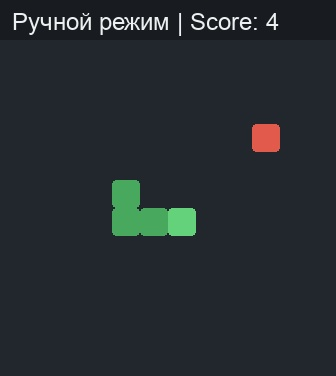
\includegraphics[width=\textwidth]{images/manual_game.jpg}
\small Ручная игра

\column{0.30\textwidth}
\centering
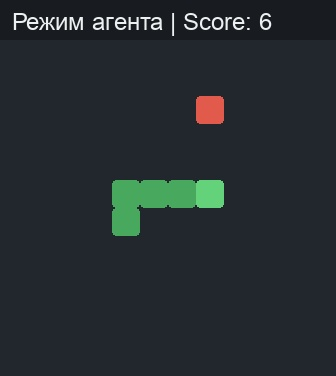
\includegraphics[width=\textwidth]{images/agent_mode.jpg}
\small Агент

\column{0.30\textwidth}
\centering
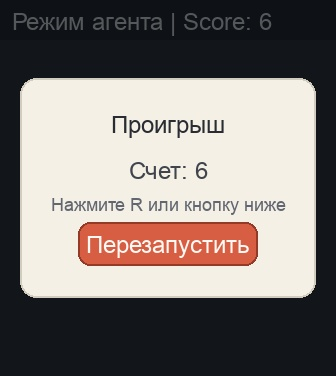
\includegraphics[width=\textwidth]{images/game_over_modal.jpg}
\small Game over
\end{columns}
\end{frame}

\begin{frame}{Методика эксперимента}
\begin{center}
\Large
5 независимых обучений $\times$ 8 вариантов $\times$ 100 тестовых игр
\end{center}

\vspace{0.4cm}
Эпизоды обучения: 50, 100, 200, 300, 500, 800, 1000, 1200

\vspace{0.3cm}
Метрика: средний score на 100 тестовых играх (без исследования)
\end{frame}

\begin{frame}{Результаты обучения}
\centering
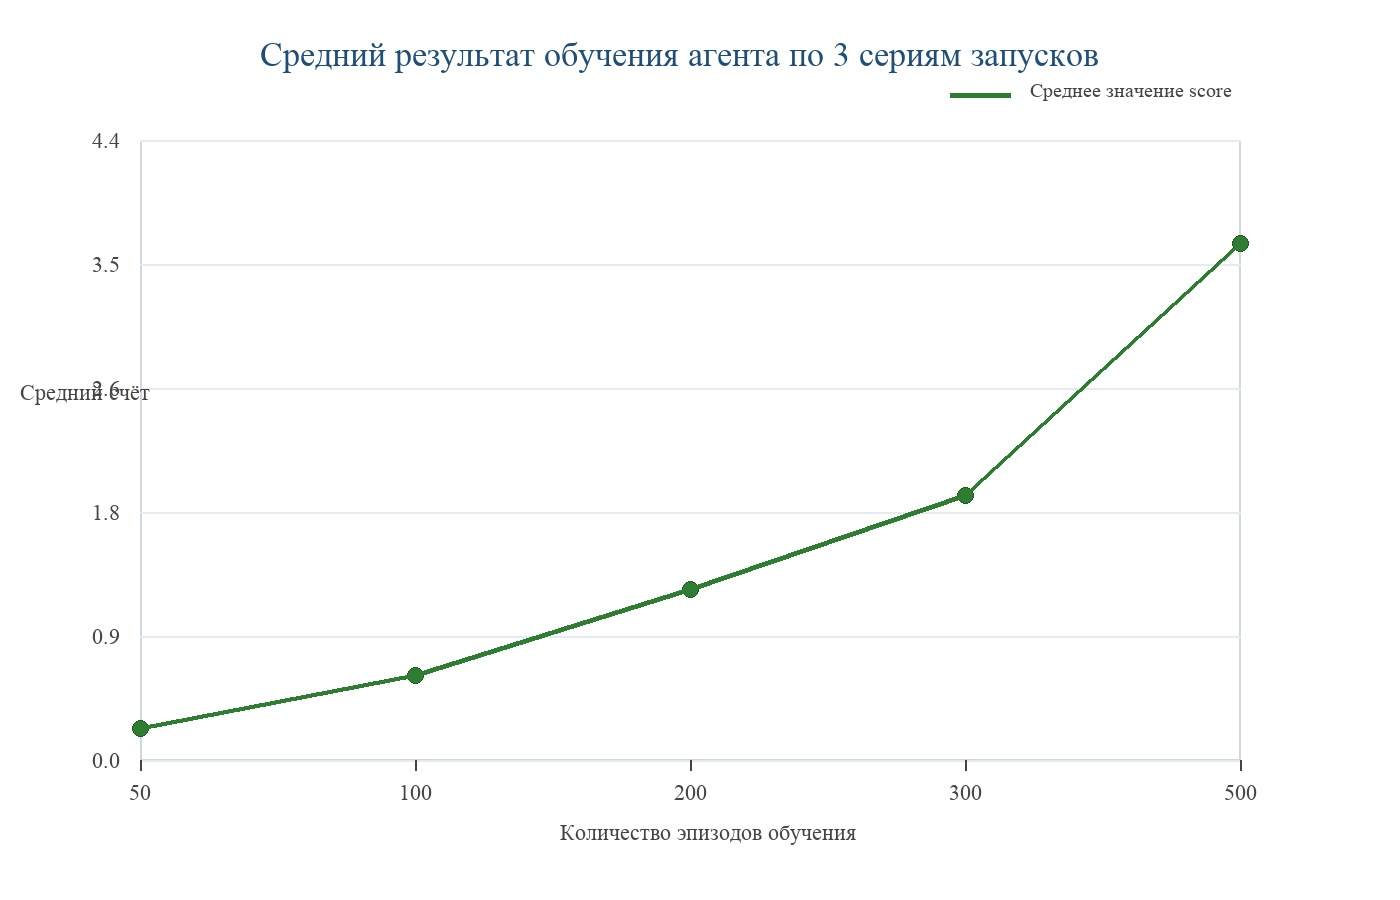
\includegraphics[width=0.85\textwidth]{images/learning_chart.jpg}
\end{frame}

\begin{frame}{Рост качества игры}
\centering
\begin{tabular}{ccc}
    \toprule
    Эпизоды & Средний score & Лучший score \\
    \midrule
    50 & 4.26 & 15.80 \\
    100 & 7.54 & 19.20 \\
    500 & 13.96 & 21.40 \\
    1200 & \textbf{16.23} & \textbf{21.60} \\
    \bottomrule
\end{tabular}

\vspace{0.5cm}
Средний score вырос с \textbf{4.26} до \textbf{16.23} --- агент усваивает стратегию.\\
После 800 эпизодов рост замедляется $\Rightarrow$ выход на плато.
\end{frame}

\begin{frame}{Выводы}
\begin{itemize}
    \setlength\itemsep{0.5cm}
    \item Цель достигнута: игра реализована, агент обучен, результаты проанализированы
    \item Табличный Q-learning формирует эффективную стратегию без нейросетей
    \item 11 бинарных признаков --- компромисс между простотой и информативностью
    \item Перспективы: влияние гиперпараметров, DQN для более сложных состояний
\end{itemize}
\end{frame}

\end{document}